\documentclass[11pt,a4paper]{article}

% ---------------------------------------------------------------- packages
\usepackage[utf8]{inputenc}
\usepackage[T1]{fontenc}
\usepackage[margin=2.5cm]{geometry}
\usepackage{amsmath,amssymb}
\usepackage{graphicx}
\usepackage{booktabs}          % \toprule etc. (used by pandas .to_latex output)
\usepackage{caption}
\usepackage{subcaption}
\usepackage{float}
\usepackage{xcolor}
\usepackage{tikz}              % Q1e protocol diagram
\usetikzlibrary{positioning,arrows.meta,shapes,fit}
\usepackage{listings}          % commands in the appendix
\usepackage[hidelinks]{hyperref}

% Figures and tables are read directly from the results folder
\graphicspath{{../results/figures/}}
\newcommand{\tablefile}[1]{\input{../results/tables/#1.tex}}

\lstset{basicstyle=\ttfamily\small,breaklines=true,frame=single,columns=fullflexible,keepspaces=true}

% ---------------------------------------------------------------- title
\title{CENG 463 -- Introduction to Machine Learning\\Take-Home Midterm Report}
\author{%
  NAME SURNAME \quad Student ID: XXXXXXXXX\\  % TODO (you)
  \small Code: \url{https://github.com/USERNAME/REPO}  % TODO (you): public link
}
\date{\today}

\begin{document}
\maketitle
\tableofcontents
\newpage

% =================================================================
\section{Introduction, research questions and datasets}
\label{sec:intro}
% TODO (you): motivation and the research questions of Q1--Q5.

\subsection{Datasets}
% TODO (you): describe both datasets (domain, target, size, feature types).
% Cite them with \cite{telco} and \cite{pace1997}.

% =================================================================
\section{Data audit, preprocessing and leakage controls}
\label{sec:audit}
% Q1a, Q1c, Q1d, Q1e.
% TODO (you): audit findings, preprocessing choices, leakage results.

% Example of including a saved table:
% \begin{table}[H]
%   \centering
%   \caption{Dataset audit (Telco).}
%   \label{tab:audit}
%   \tablefile{telco_audit}
% \end{table}

% =================================================================
\section{Methods and experimental design}
\label{sec:methods}
% Q1--Q5: models, pipelines, what is compared and why.
% TODO (you)

% Protocol diagram (Q1e) goes here (TikZ figure).

% =================================================================
\section{Validation scheme, tuning grids, random seeds and computing environment}
\label{sec:validation}

\begin{table}[H]
  \centering
  \caption{Exact split sizes, Telco Churn (stratified on \texttt{Churn}). \texttt{target\_mean} is the churn rate.}
  \label{tab:clf_split_sizes}
  \tablefile{clf_split_sizes}
\end{table}

\begin{table}[H]
  \centering
  \caption{Exact split sizes, California Housing (random). \texttt{target\_mean} is the mean \texttt{MedHouseVal} ($\times$100{,}000 USD).}
  \label{tab:reg_split_sizes}
  \tablefile{reg_split_sizes}
\end{table}

% TODO (you): describe the validation scheme (60/20/20, 5-fold StratifiedKFold
% on train, Macro-F1 selection, seed 463, test set used once).
% Tuning-grid table per model goes here.

\paragraph{Computing environment.}
Windows 11 Home, Intel Core i7-13650HX (20 logical cores), 15.7\,GB RAM, no GPU.
Python 3.12.7, scikit-learn 1.9.1, NumPy 2.5.5, pandas 3.1.1,
imbalanced-learn 0.14.2, matplotlib 3.11.2, seaborn 0.13.2.

% =================================================================
\section{Results and interpretation}
\label{sec:results}
% Labelled tables and figures for Q1--Q5, each followed by YOUR interpretation.
% Figure example:
% \begin{figure}[H]
%   \centering
%   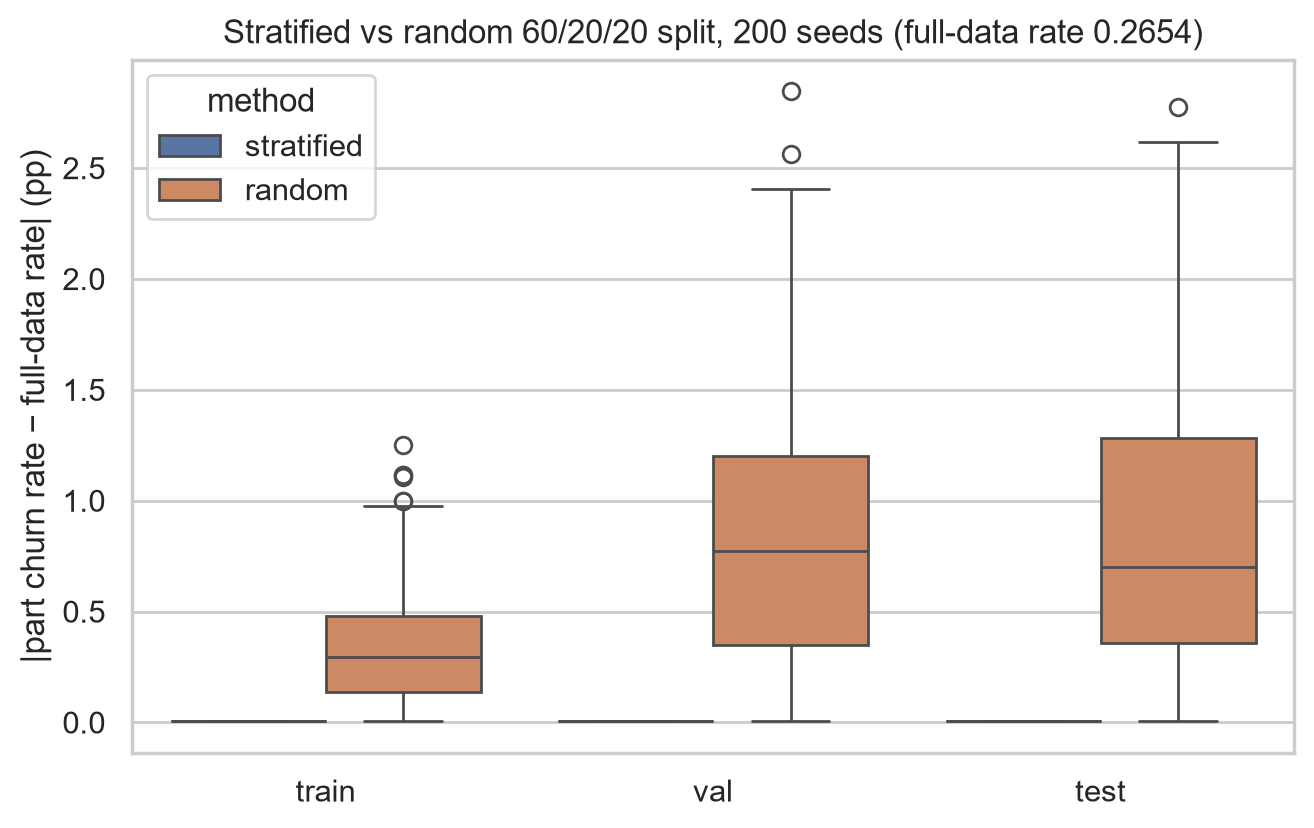
\includegraphics[width=0.7\linewidth]{q1b_split_deviation_boxplot}
%   \caption{...}
%   \label{fig:q1b}
% \end{figure}
% TODO (you)

\subsection{Q1 -- Data preparation and leakage}
\subsection{Q2 -- Classification and error analysis}
\subsection{Q3 -- Regression, regularization and generalization}
\subsection{Q4 -- Decision trees, bagging and boosting}
\subsection{Q5 -- Robustness and statistical comparison}

% =================================================================
\section{Error analysis, robustness, uncertainty and limitations}
\label{sec:error}
% Q2e, Q3e, Q5b, Q5c.
% TODO (you)

% =================================================================
\section{Final model-selection rationale and test-set evaluation}
\label{sec:final}
% Q5d, Q5e: frozen configurations, selection rule, single test evaluation.
% TODO (you)

% =================================================================
\section{LLM Usage Disclosure}
\label{sec:llm}
% Required by the exam. Use LLM_USAGE_LOG.md as the source.
% TODO (you): tool and model, purpose (code writing, debugging, environment
% setup), example prompts, and confirmation that interpretation/discussion
% text and all reported results are your own.

% =================================================================
\section{References and reproducibility appendix}
\label{sec:repro}

\subsection*{Reproducing the results}
\begin{lstlisting}
git clone https://github.com/USERNAME/REPO
cd REPO
python -m venv .venv
.venv\Scripts\Activate.ps1        (Windows)  /  source .venv/bin/activate
pip install -r requirements.txt
# run notebooks/00 ... 05 in order with Restart & Run All
\end{lstlisting}

\begin{itemize}
  \item Random seed: \texttt{SEED = 463} (NumPy, \texttt{random\_state} of all scikit-learn objects, bootstrap, corruptions).
  \item Split indices: \texttt{results/splits/clf\_split\_indices.csv}, \texttt{results/splits/reg\_split\_indices.csv}.
  \item Cross-validation: \texttt{StratifiedKFold(n\_splits=5, shuffle=True, random\_state=463)} (classification), \texttt{KFold} with the same settings (regression).
  \item Frozen configurations before the final test: \texttt{results/frozen\_configs.json}.
\end{itemize}

\nocite{*}  % TODO: remove once all references are cited in the text
\bibliographystyle{plain}
\bibliography{references}

\end{document}
